\section {Image Recognition}
Image recognition is a very interesting topic in computer vision and pattern recognition, and the goal is to recognize different classes in images. For instance, there are trees, people, sun, moon and buildings in different images. Human can easily distinguish different classes among a set of images. However, machines are not good at such tasks. For many years, a lot of researchers are working on this topic and have achieved significant results.\\

\noindent So far, a very good framework to recognize images is the so-called {\em bag of words} model, which generalizes from natural language processing (NLP). In NLP, bag of words basically aims to represent an article using histogram of word frequencies. Following this idea, in image recognition, an image is also represented as a histogram of visual words, and these visual words normally come from centroids generated from clustering algorithms. Later on, such representations of images are used to build up generic machine learning models, and the accuracy is quite impressive. During recognition phase, the most critical process is to calculate image-to-image distance. One direct way is the Euclidean distance. But a better way to calculate distance is called as Earth Mover's Distance \cite{rubner2000earth}, which finds the best matches between image parts and produces a more accurate distance. \\

\noindent In the following of this section, an image recognition framework consisting of 4 steps is first introduced. Secondly, Earth Mover's distance and its applications in image recognition is talked about. Lastly, the method to identify duplicates in a cluster of images used in this project are presented, and this method is going to be applied in video recognition to show the effectiveness of Earth Mover's distance.

\subsection{Framework Description}

Generally, there are 4 below steps to go:

\subsubsection{Extract SIFT features from each image}
It is almost impossible to directly rely on pixel data of images to perform recognition tasks, and the main reason is because such pixel data does not possess much discriminative power. Therefore, other approaches to represent images are needed. One approach is to extract features from images and use those features to represent images compactly. There are generally two categories of features: global features and local features. As the name stated, global features encode a whole image based on the overall distribution of color, texture, or edge information. Some popular global features include color histogram and Gabor texture \cite{manjunath1996texture}. On the other hand, local features refer to features extracted from local patches (or interest points). There are two steps involved in extracting local features: detection and description. Detection refers to localizing interest points in images. Among popular detection algorithms, the most widely used is Difference-of-Gaussian (DOG) \cite{lowe2004distinctive} introduced by David Lowe, which detects blob regions where the centroids differs from their neighbors. Other popular detectors include Harris-Laplace \cite{lindeberg1998feature}, Hessian \cite{mikolajczyk2004scale}, etc. The next stage is description which aims to describe those located interest points in meaningful manners such that this descriptor is invariant to scale, viewpoint, rotation and illumination changes. There are lots of descriptors that have been designed over years. The best known shall be Scale Invariant Feature Transform (SIFT) \cite{lowe2004distinctive}, which concatenates histograms of gradient orientation around interest points. Other descriptors include Histogram of oriented gradients (HOG) \cite{dalal2005histograms}, Local binary pattern (LBP) \cite{ojala2002multiresolution}, etc. Given the robustness of SIFT shown in various literatures \cite{duan2012visual,zhou2008sift,lazebnik2006beyond, lowe2004distinctive}, SIFT is chosen to be the feature to be extracted from images through the whole period of this project.\\

\noindent Now it's time to briefly elaborate details about SIFT. There are two steps when performing extracting SIFT features. The first step is to identify interest points, and the criteria is based on {\em difference-of-Gaussian functions}:
\begin{equation}
D(x, y, \sigma) = (G(x, y, k\sigma) - G(x, y, \sigma)) * I(x, y)
\end{equation}

\noindent where $G$ is the Gaussian 2D kernel, $I(x, y)$ is an input image and $k$ is a constant multiplicative factor which separates two nearby scales. After computing $D(x, y, \sigma)$ for all sample points, those sample points with local maxima and minima of $D(x, y, \sigma)$ compared with their neighbors are selected to be interest points. In order to better localize interest points, these candidate locations are filtered to remove unstable points based on criteria including low contrast and edge response. Please refer to the paper \cite{lowe2004distinctive} for details on removing unstable points. The next step is to compute a descriptor based on those interest points located in previous step. For each interest point, a descriptor is created by first computing the gradient magnitude and orientation in a grid of subregions around that specific interest point. These gradient orientations are then accumulated into orientation histograms. Finally, these histograms are concatenated to form a descriptor vector. The recommended setting uses $4 \times 4$ subregions with 8 bin histogram, which results in a 128 bin histograms ($4 \times 4 \times 8 = 128$). Figure 1 below demonstrates the whole process to construct SIFT descriptor. \\

\begin{figure}[!ht]
\centering
  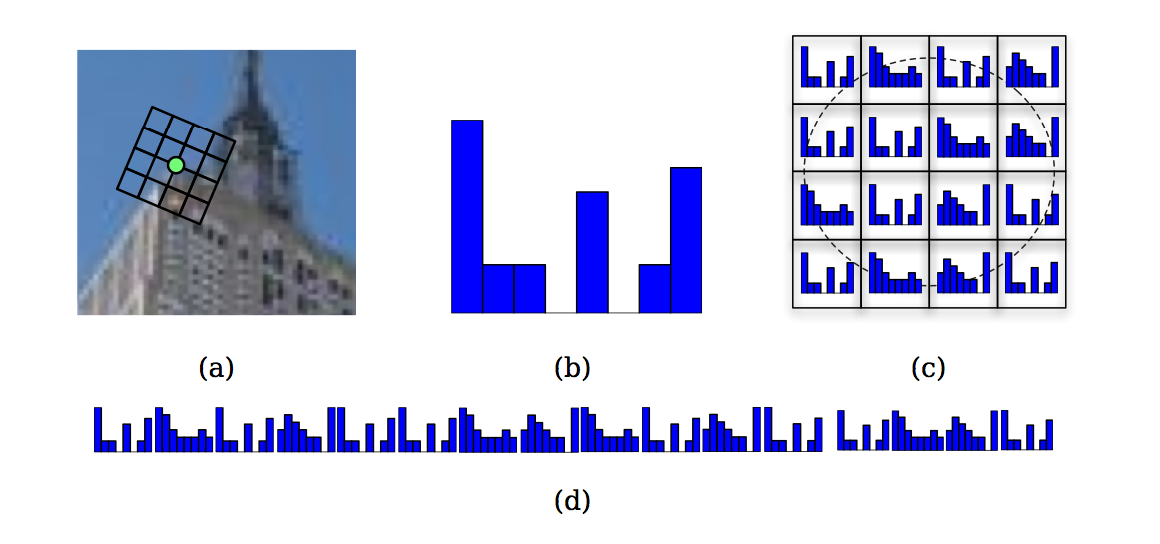
\includegraphics[width=1\textwidth]{./SIFT_Descriptor.png}
\caption{SIFT descriptor \cite{solem2012programming} (a) a frame with $4 \times 4$ subregions around an interest point. (b) an 8 bin histogram over the direction of gradient in one subregion. (c) all histograms in their respective subregions. (d) all 16 histograms are concatenated to form a 128 ($16 \times 8$) dimensional vector.}
\end{figure}

\noindent For simplicity, an open source library VLFEAT \cite{vedaldi08vlfeat} is adopted to extract SIFT from images. A typical image of size $200 \times 200$ normally produces around 800 SIFT features.  

\subsubsection{Build up visual vocabulary from features of training set}
Although SIFT features have been extracted, these 128 dimensional raw features are still not an ideal representation because of limitations including the curse of dimensionality. Thus, a visual vocabulary is needed to map high dimensional descriptors to words by quantizing the feature space. Commonly, vocabulary is built through applying K-Means \cite{lloyd1982least} clustering algorithm on available features, and the final centroids output by K-Means are treated as representative words. The basic K-means algorithm goes as below:

\begin{algorithm}
  \caption{Basic K-means Algorithm}
  \begin {algorithmic}[1]
  \State Randomly select K points as the initial centroids
  \Do 
    \State Form K clusters by assigning all points to their closest centroids.
    \State Recompute the centroid of each cluster
  \doWhile Centroids are changed
  \end{algorithmic}
\end{algorithm}

\noindent Based on the above algorithm, it is easy to see that the time complexity is $O(n*K*I*d)$, where $n$ is the number of points, $K$ is the number of clusters, $I$ is the number of iterations and $d$ is the number of dimensions. This classical K-means algorithm works fine for small data sets but is very expensive for large data sets. Later on, vocabulary is also needed for video recognition where the number of features is nearly 0.4 million after sampling. By noticing that the available computational resource is limited, it is not affordable to apply classical K-Means on large data sets. Therefore, a better method is needed to build up vocabularies.  Mini-Batch K-Means \cite{sculley2010web}, a variant of KMeans algorithm which uses mini-batches to reduce the computation time, is a good alternative. In contrast to other algorithms which reduce the convergence time of k-means, mini-batch k-means produces results that are generally only slightly worse than the standard algorithm. The details about mini-batch k-means are presented as follows:

\begin{algorithm}
  \caption{Mini-batch K-Means}
  \begin{algorithmic}[1]
  \State Given: $k$, mini-batch size $b$, iteration $t$, data set $X$
  \State Initialize each $c \in C$ with an $x$ picked randomly from $X$
  \State $v \gets 0$
  \For {$i = 1$ to $t$}
  \State $M \gets b$ examples picked randomly from $X$
  
  \For {$x \in M$}
  \State $d[x] \gets f(C, x)$ \Comment{Cache the nearest center to $x$}
  \EndFor

  \For {$x \in M$}
  \State $c \gets d[x]$ \Comment{Get cached center for this $x$}
  \State $v[c] \gets v[c] + 1$ \Comment{Update per-center counts}
  \State $\eta \gets \frac{1}{v[c]}$ \Comment{Get per-center learning rate}
  \State $c \gets (1 - \eta)c + \eta x$ \Comment{Take gradient step}
  \EndFor
  
  \EndFor
  \end{algorithmic}
\end{algorithm}

\noindent Once this vocabulary is built, a histogram whose length equals to the size of vocabulary is built for each image. Afterward, features of images are examined to construct their histograms. For each SIFT feature, the nearest word to this feature is found, and the bin representing the found word is increased by one. After finishing examining all features, a histogram is constructed and is used to represent the respective image. As a result, all images are transformed from pixels to fixed length histograms. In image recognition experiments, the number of centroids is set to be 300 when performing Mini-Batch K-Means. Thus, all images are converted into 300 dimensional histograms. 

\subsubsection{Construct a pyramid of three levels for each image}
Now that histograms for images are built, these histograms could be put into machine learning models including K Nearest Neighbor and Support Vector Machine for recognition. However, this is not the end of story. To enable more discriminative power, Grauman and Darrell \cite{grauman2005pyramid} proposed {\em pyramid matching} in 2005 to find an approximate correspondence between 2 sets of data. The basic idea is to map sets of features to multi-resolution histograms, and then compare the histograms with a weighted histogram intersection measure in order to better approximate the similarity of best partial matching. As reported in the paper \cite{grauman2005pyramid}, this pyramid match kernel produces much better recognition results for similar running time. \\

\noindent Though {\em pyramid matching} fuses information from multiple levels built on different resolutions, this method ignores spatial information because features are matched without any order. To partially address this problem, in the following year, Lazebnik introduced spatial pyramid matching \cite{lazebnik2006beyond}. Unlike pyramid matching which varies histogram matching resolution, spatial pyramid matching varies the spatial resolution at which they are aggregated. Figure 2 below demonstrates the case when there are three levels in spatial pyramid matching. The three levels are presented from the left to right. Level 0 is simply a standard bag of features which treats the whole image as a whole. For level 1, this image is divided equally into 4 parts, each part contributes to one histogram built on the same vocabulary. Furthermore, level 2 is the case when image is divided into 16 parts which results in 16 different histograms. Finally, all these histograms are concatenated with appropriate weights to form a ``long'' histogram with dimensionality as $M\sum_{l=0}^{L}4^{l}$, where $M$ is the size of vocabulary and $L$ equals to total number of levels $ - 1$. For instance, the vocabulary size used in experiments is 300. Thus, the number of dimensions is 1500 for two-level spatial pyramid and 6300 for three-level spatial pyramid. Additionally, the weights for histograms at different levels are listed below:

\begin{equation}
 weight(l) = \left\{ 
\begin{array}{l l}
  \frac{1}{2^L} & \quad \text{$if \ l = 0$ }\\
  \frac{1}{2^{L-l+1}} & \quad \text{$Otherwise$}
\end{array} \right.
\end{equation}

\noindent For example, as shown in Figure 2, weights for three levels histograms are $\frac{1}{4}$, $\frac{1}{4}$ and $\frac{1}{2}$, respectively. It is easy to see that such weighting scheme tends to penalize matches found in larger cells, and the reason why it makes sense is because larger cells allow more dissimilar features. 

\begin{figure}[!ht]
\centering
  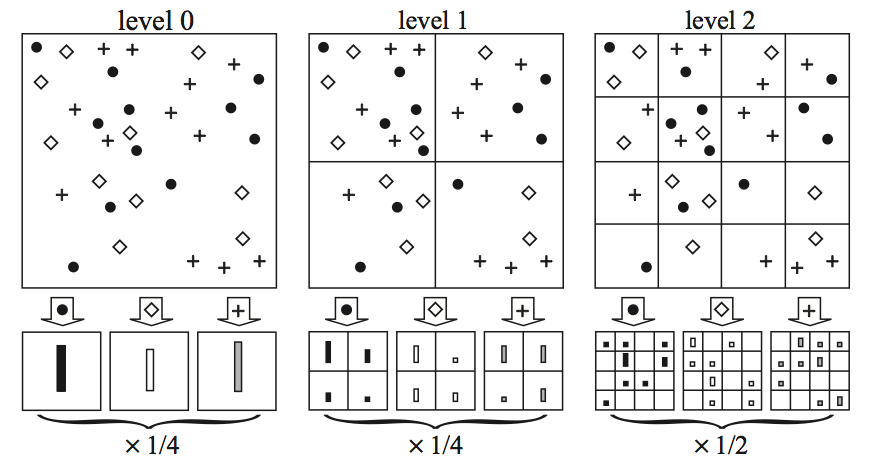
\includegraphics[width=1\textwidth]{./SpatialPyramidMatch.png}
\caption{Example to construct a three-level pyramid \cite{lazebnik2006beyond}. At top, images are divided at three different levels of resolution. Next, the count to each feature is calculated for each spatial bin. Finally, each histogram is weighted according to equation (2)}
\end{figure}

\subsubsection{Classify based on above representations}
In machine learning, classification refers to the problem of identifying to which category a new observation belongs, on the basis of training data set. Generally, machine learning builds a model which fits the training data set. Afterward, this model to use to recognize new data set. There are many classification methods including K-nearest neighbors (KNN), support vector machine (SVM), decision tree, etc. In this project, KNN and SVM are incorporated into the recognition system, and details about these two kinds of classification methods will be presented in following paragraphs. 

  \paragraph{K-nearest neighbor (KNN)} 
  K-nearest neighbor is considered as a lazy learning algorithm. This is because it does not attempt to construct a general internal model, but just store all instances of the training data. Once a test case is input, KNN retrieves the nearest $K (K>0)$ neighbors to this test case from training data, and the predicted label is computed based on labels of neighbors in a majority vote manner. In other words, the predicted label of a test case is chosen to be the most representative label among $K$ nearest neighbors. For example, Figure 3 shows how to predict label for $x_{q}$ when $K$ is set to be 5. Among 5 neighbors of $x_{q}$, three are negative while the left two are positive. Therefore, $x_{q}$ is predicted to be within negative class based on majority vote. 

  \begin{figure}[!ht]
  \centering
    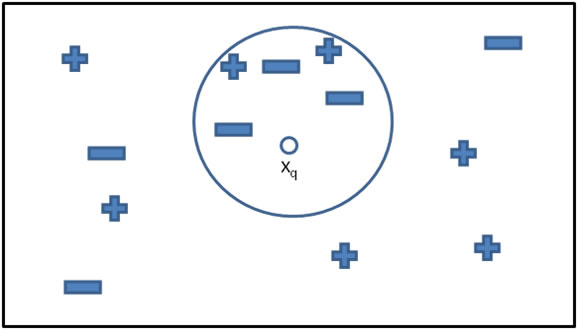
\includegraphics[scale=0.5]{./knn.jpg}
  \caption{A case of k nearest neighbor. Among 5 neighbors of $x_{q}$, three are negative while the other two are positive. As a result, the label of $x_{q}$ is predicted to be negative.}
  \end{figure}

  \paragraph{Support vector machine (SVM)}
  Support Vector Machine was introduced in COLT-92 by Boser, Guyon \& Vapnik \cite{boser1992training} and became rather popular since then. This is a well motivated algorithm which is developed from statistical learning theory since 1960s. It has been successfully applied into many fields (bioinformatics, text, image recognition, ...) and is currently the most popular classifier in event recognition systems \cite{jiang2012high}. \\

  \noindent SVM starts with the problem of finding the optimal separating hyperplane which separates a linearly separable dataset: $${(x_{1}, y_{1}), (x_{2}, y_{2}), ..., (x_{n}, y_{n})}$$ where $x \in R^{D}$ and $y \in  \{ -1, +1 \}$. An example is presented in Figure 4. Black solid circle represents one class while the while circle represents another class. The solid line $\mathbf{w} \mathbf{x} + b = 0$ is the optimal hyperplane, and the data points on $\mathbf{w} \mathbf{x} + b = 1$ and $\mathbf{w} \mathbf{x} + b = -1$ are called are {\em support vectors}. It is not difficult to see that the distances from support vectors to optimal hyperplane  are maximized. Therefore, the finding of optimal hyperplane is transformed into an optimization problem:
  \begin{eqnarray}
  & \text{minimize} \quad J(\mathbf{w}) = \frac{1}{2} \norm{\mathbf{w}}^2 \nonumber \\
  & \text{subject to} \quad y_i (\mathbf{w}^{T} x_i + b) \ge 1 \quad \forall i
  \end{eqnarray}
  
  \begin{figure}[!ht]
  \centering
    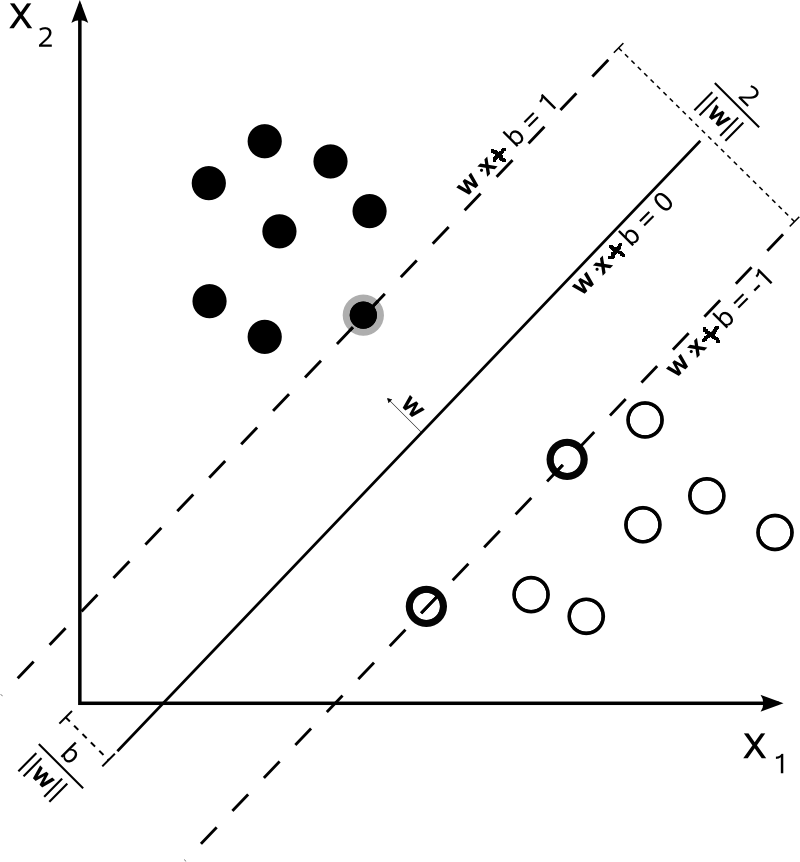
\includegraphics[scale=0.3]{./svm.png}
  \caption{Optimal hyperplane which separates a linearly separable dataset}
  \end{figure}

  \noindent This optimization is generally solved by introducing the Lagrangian:
  \begin{equation}
  L(w,b,\alpha) = \frac{1}{2} \norm{w}^2 - \sum_{i = 1}^{N} \alpha_i [ y_i ( w^T x_i + b) - 1 ]
  \end{equation} 
  where $\alpha_i$ are dual variables. After substituting stationary conditions, the Lagrangian gives the dual cost function:
  
  \begin{equation}
  W(\alpha) = \sum_i \alpha_i - \frac{1}{2} \sum_{i,j} y_i y_j \alpha_i \alpha_j x_i^{T} x_j
  \end{equation}

  \noindent The optimization is now:
  \begin{eqnarray}
  & \hat{\alpha} = \argmax{\alpha} W(\alpha) \nonumber\\
  & \text{subject to} \quad \alpha_i \ge 0  \quad \text{and} \quad \sum_{i=1}^{N} \alpha_i y_i = 0
  \end{eqnarray}

  \noindent So far, the problem of finding s saddle point for $L(w, b)$ becomes an easier one of maximizing $W(\alpha)$. Once this optimization problem is solved, the decision function to predict new data points is shown as follows:

  \begin{equation}
  f(x) = \text{sign}\bigg(\sum_i y_i \alpha_i x_i^T x + b\bigg)
  \end{equation}
  Please note that in equation (7), the point set $\{x_i\}$ includes all calculated support vectors. Moreover, the training data appears as dot products $x_i^T x_j$ in $W(\alpha)$, and it means that classification could be done in higher or even infinite dimensional space by changing $x_i^T x_j$ into other forms of kernel function. Suppose there is a kernel function $K(x, y)$, the original optimization problem is converted by replacing $x_i^T x_j$ with $K(x_i, x_j)$:

  \begin{equation}
  W(\alpha) = \sum_i \alpha_i - \frac{1}{2} \sum_{i,j} y_i y_j \alpha_i \alpha_j K(x_i, x_j)
  \end{equation}

  \noindent Because this transformation has nothing to do with $\alpha_i$ and $y_i$, the optimization remains the same:
  \begin{eqnarray}
  & \hat{\alpha} = \argmax{\alpha} W(\alpha) \nonumber\\
  & \text{subject to} \quad \alpha_i \ge 0  \quad \text{and} \quad \sum_{i=1}^{N} \alpha_i y_i = 0
  \end{eqnarray}
  Finally, the decision function becomes:

  \begin{equation}
  f(x) = \text{sign}\bigg(\sum_i y_i \alpha_i K(x_i,x) + b\bigg)
  \end{equation}
  As shown above, thanks to the kernel function $K(x_i, x_j)$, nonlinear classification is achieved without projecting data points into higher dimensional space. This clever trick refers to ``kernel trick''. Detailed information can be found at \cite{burges1998tutorial}. \\

  \noindent There are many kernels designed over years, and different kernels have different impacts on recognition performances. In experiments of image recognition, the below four kernel functions have been implemented.
  
    \begin{table}[!ht]
        \begin{center}
        \scalebox{1}{
          \begin{tabular}{cc}
          \hline
          \head{Kernel type} & \head{Kernel function}\\
          \hline
          Linear & $x_i^T x_j$ \\
          Polynomial & $(\gamma x_i^T x_j + r)^d$ \\ 
          RBF & $\exp(-\gamma \norm{x_i - x_j}^2)$ \\ 
          Sigmoid & $\tanh(\gamma x_i^T x_j + r)$ \\ 
          Histogram intersection \cite{barla2003histogram} &  $\sum_{p = 1}^{D} min(x_i^p, x_j^p)$ \\
          \hline
          \end{tabular}
        }
        \end{center}
        \caption{Kernel functions}
    \end{table}

  \noindent Although the above mathematical description of support vector machine seems to be complex, there are lots of open source libraries of SVM. One famous and popular package is LIBSVM \cite{CC01a}. What's better is that sklearn \cite{scikit-learn} provides well defined python wrapper to invoke LIBSVM. All the work facilitates the use of SVM, and it demonstrates the collaboration among researchers all around the world.

\subsection{Earth Mover's Distance (EMD)}
In this subsection, Earth mover' distance will be introduced, and the reason is because later on in video recognition, this kind of distance calculation is going to be heavily used. The rest of this section is organized as follows. Firstly, the mathematical model of earth mover proposed by Rubner, Tomasi and Guibas \cite{rubner2000earth} is presented followed by an example of calculating earth mover distance between two images. Last but not least, experiments have been done to show the effectiveness of EMD, and the result is recorded in the section of experiments.\\

\noindent The earth mover's distance is formulated as the following linear programming problem: Let $P = \{(p_1, w_{p_1} ), . . . , (p_m , w_{p_m} )\}$ be the first signature with $m$ clusters, where $p_i$ is the cluster representative and $w_{pi}$ is the weight of the cluster; $Q=\{(q_1,w_{q_1}),...,(q_n,w_{q_n})\}$ the second signature with $n$ clusters; and $D = [d_{ij}]$ the ground distance matrix where $d_{ij}$ is the ground distance between clusters $p_i$ and $q_j$. We want to find a flow $F = [f_{ij}]$, with $f_{ij}$ being the flow between $p_i$ and $q_j$, that minimizes the overall cost: 
\begin{eqnarray}
\text{minimize} & Work(P , Q, F) = \sum_{i=1}^{m}\sum_{j=1}^{n}d_{ij}f_{ij} \nonumber\\
\text{subjective to } & f_{ij} \geq 0 \quad \quad 1 \leq i \leq m,  1 \leq j \leq n \nonumber\\ 
& \sum_{j=1}^n f_{ij} \leq w_{p_i} \quad 1 \leq i \leq m \nonumber\\
& \sum_{i=1}^m f_{ij} \leq w_{q_j} \quad 1 \leq j \leq n \nonumber\\
& \sum_{i=1}^{m} \sum_{j=1}^n f_{ij} = min(\sum_{i=1}^m w_{p_i}, \sum_{j=1}^n w_{q_j}) 
\end{eqnarray}

\noindent Once the above linear programming problem is solved, the earth mover's distance is defined as the resulting work normalized by the total flow:
\begin{equation}
EMD(P, Q) = \frac{\sum_{i=1}^m \sum_{j=1}^n d_{ij} f_{ij}}{\sum_{i=1}^m\sum_{j=1}^n f_{ij}}
\end{equation}

\begin{figure}[!ht]
\centering
	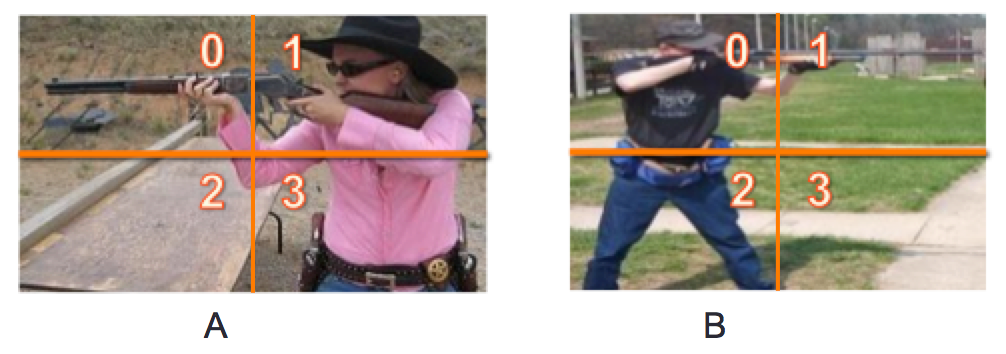
\includegraphics[width=1\textwidth]{./image_EMD_Sample.png}
\caption{Image $A$ and $B$ are divided into 4 parts equally. Then each part is converted into a histogram. Thus, four histograms are stacked to represent each image.}
\end{figure}

\noindent To better understand EMD, here is an example to incorporate EMD into the distance calculation of images. To do so, the first step is to divide each image into four parts equally. An example is depicted in Figure 5. There are two images $A$ and $B$, and they are both divided into 4 parts equally. Each part is then represented by a histogram based on previous built vocabulary. It is easy to see that this division is identical to level 1 in spatial pyramid matching, which also divides an image into 4 equal parts. Now image $A$ and $B$ are represented by 4 histograms each. After adding equal signature value to these histograms, $A$ and $B$ are represented as follows:
	$$A = \{(a_0, 0.25), (a_1, 0.25), (a_2, 0.25), (a_3, 0.25)\}$$
	$$B = \{(b_0, 0.25), (b_1, 0.25), (b_2, 0.25), (b_3, 0.25)\}$$
where $a_0, a_1, a_2, a_3$ and $b_0, b_1, b_2, b_3$ are histograms generated from respective parts.\\

\noindent The next steps is to calculate the distance matrix $D$ with each cell $d_{ij}$ representing the distance between $a_i$ and $b_j$. In this case, Euclidean distance is adopted, and the calculated distance matrix is shown below in Table 2.

\begin{table}[!ht]
    \begin{center}
    \scalebox{0.8}{
      \begin{tabular}{ccccc}
      \hline
      \head{} & \head{$b_0$} & \head{$b_1$} & \head{$b_2$} &\head{$b_3$} \\
      \hline
      $a_0$ & 27.06473721	& 23.37733946	& 29.18047292 &	32.61901286\\
    	$a_1$ & 20.84466359	& 21.50581317	& 21.70253441 &	30.34798181\\
    	$a_2$ & 26.48584528	& 27.38612788	& 27.46816339 &	34.71310992\\
    	$a_3$ & 19.31320792	& 24.20743687	& 21.59861107 &	31.81194744\\
      \hline
      \end{tabular}
    }
    \end{center}
    \caption{Distance matrix between image $A$ and $B$}
\end{table}

\noindent If EMD is not used meaning that there is no alignment of image segments, $a_0$ is matched to $b_0$, $a_1$ is matched to $b_1$, $a_2$ is matched to $b_2$ and $a_3$ is matched to $b_3$. As a result, distance without alignment is calculated as below: $$distance_{unaligned} = d_{00} + d_{11} + d_{22} + d_{33} = 107.851$$

\noindent However, if EMD is used, the best matches between image segments will be found after the linear programming problem in EMD is solved. For image $A$ and $B$, the best matches found are shown in Figure 6. Compared with unaligned case, this one matches the gun and human body properly. Following the matches in Figure 6, distance with alignment is calculated as below: $$distance_{aligned} = d_{30} + d_{12} + d_{01} + d_{23} = 99.106$$

\begin{figure}[!ht]
\centering
	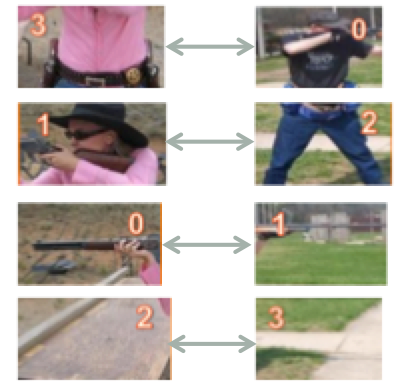
\includegraphics[scale = 1]{./image_EMD.png}
\caption{Matches between segments of $A$ and $B$ calculated by EMD. As we can see, the gun, human body and ground are matched properly. Therefore, distance with alignment shall be more accurate.}
\end{figure}

\noindent Now that the calculation of distances between images  has been defined, it is needed to select a kernel type for SVM to recognize. Apart from RBF (also called as Gaussian kernel) introduced before, three more kernel types were tried in experiments, and they are listed in Table 3. Details of performances of these four kernel types are presented in the experiment section. 
\begin{table}[!ht]
    \begin{center}
      \begin{tabular}{cc}
      \hline
      \head{Kernel type} & \head{Kernel function}\\
      \hline
      Gaussian & $\exp(-\gamma D^2(I_i, I_j)$ \\
      Laplacian & $\exp(- \sqrt{\gamma} D(I_i, I_j)$ \\
      ISD & $\frac{1}{\gamma D^2(I_i, I_j) + 1}$ \\
      ID & $\frac{1}{\sqrt{\gamma}D(I_i, I_j) + 1}$\\
      \hline
      \end{tabular}
    \end{center}
    \caption{Four kernel types which have been tested. $D(I_i, I_j)$ represents the distance between $I_i$ and $I_j$. The kernel parameter $\gamma$ is selected to be the default one $\gamma = \frac{1}{A}$, where $A$ is the mean value of the squared distances between training samples as suggested in \cite{laptev2008learning}.} 
\end{table}

\subsection {Key Frame Identification in a Cluster of Images}
A video could be simplified as a cluster of consecutive frames. By noticing that some consecutive frames in video are similar to each other, it is thought that video can be described by several key frames. In doing so, the data to represent each video can thus be largely reduced. One key step in key frame identification is to check whether two images are near duplicate. If two or more images are examined to be near duplicate to each other, only one image will be selected to represent these images. The rest of this section will focus on two parts: near duplicate identification and how to apply near duplicate identification into key frame identification in videos.

\subsubsection{Identifying near duplicate}
The way which has been implemented to check whether two images are near duplicate follows the method stated on paper \cite{zhao2007near}. In this paper, there are basically three steps to check whether two images are near duplicates. Firstly, the authors propose to use a hash table to match SIFT points. Secondly, a SVM classifier is built based on the matching SIFT points. Finally, this classifier could be used to check near duplicates. Due to a lack of training set, the classifier is not built and thus has to be replaced by threshold checking. In other words, two images are treated as near duplicates as long as the number of matching interest point is large enough compared with a predefined threshold. \\

\noindent In order to minimize false matches, the authors propose one-to-one symmetric matching \cite{zhao2007near}, which ensures all the matches are nearest neighbors. One the other hand, the symmetric property makes sure that the matching result of set A to B is exactly the same as B to A. Suppose there are two images $I_1$ and $I_2$, the steps to check whether these two images are near duplicate go as below:

\begin{enumerate}
  \item{\bfseries Perform PCA on SIFT features of $I_1$ and $I_2$ to reduce dimensions}
  The dimension of SIFT feature is reduced from 128 to 36, and each value of reduced feature is normalized to be within the range [0, 2]. 

  \item{\bfseries Hash all interest points of $I_1$ into a $8 \times 36$ table}

  \begin{figure}[!ht]
  \centering
    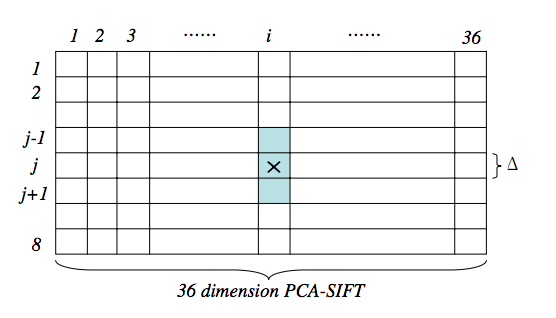
\includegraphics[scale = 0.8]{./hashTable.png}
  \caption{$8 \times 36$ Hash Table \cite{zhao2007near}}
  \end{figure}
  
  The hash table is composed of $8 \times 36$ bins as shown in Figure 7. Given each point $P = [p_1, p_2,..., p_{36}]$ of $I_1$, the index of $p_i$ is hashed to, 
  $$H(p_i) = \lfloor p_i \times 4 \rfloor$$ 
  Since the dimension is 36, $P$ is repeatedly indexed into the corresponding bin for 36 times, according to its quantized value in a particular dimension.   
  
  \item{\bfseries For each interest point $Q$ of $I_2$, examine whether there is a match in $I_1$}\\
  There are three sub steps to go:
    
    \begin{enumerate}
    \item {Hash $Q$ into the hash table}
    \item {Retrieve the set $A(Q)$ satisfying the below constraints}\\
    For each interest point $P \in I_1$, put $P$ into $A(Q)$ if $$\sum_{i=1}^{36}f(q_i, p_i) = 36$$ 

    where 
    \begin{equation*}
        f(q_i, p_i) = \begin{cases}
                   1     & \text{if } \left|H(q_i) - H(p_i)\right| \leq 1\\
                   0 & \text{otherwise}
               \end{cases}
    \end{equation*}

    \item {If $A(Q)$ is not empty, find the nearest neighbor $M \in A(Q)$ with one-to-one symmetric constraint as $Q$' match}
    \end{enumerate}

  \item{\bfseries If the number of matching interest point is large enough, $I_1$ and $I_2$ are near duplicates}
\end{enumerate}

\noindent An example of performing the above algorithm is depicted below in Figure 8. Those colored lines in the upper two images connect the matched interest points, and it is easy to distinguish that the matching accuracy is quite high because of one-to-one constraint \cite{zhao2007near}. Please also notice that only partial matching points are drawn for better visualization. 
  \begin{figure}[!ht]
  \centering
    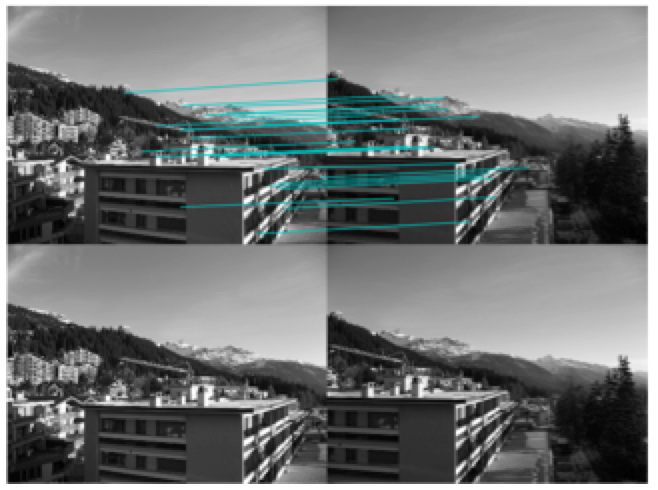
\includegraphics[]{./match.png}
  \caption{Near duplicate example. The colored lines in upper two images connect partial matched interest points, and the below two images are original images.}
  \end{figure}

\subsubsection{Identifying key frames} 
Now that near duplicate method is introduced, it is time to check how this method could be incorporated into key frame identification. The naive brute-force identification checks any two frames in a video, and the computational cost is $O(cn^2)$, where $c$ is the cost of identification and $n$ is the number of all frames. Because $c$ is almost fixed, the left way to reduce computational time is to reduce $n$. Inspired by the paper \cite{wang2012event}, it is recommended to perform K-means algorithm on all the frames at first. Later on, the previous introduced near duplicate identification is performed within each cluster. In this case, if all clusters have equal size, the cost becomes $O(cn^2/r)$, where $r$ is the number of clusters.\\

\noindent Once the clusters are calculated through K-means, the steps to identify key frames in each cluster go as below:

\begin{enumerate}
  \item{\bfseries Build a graph for each cluster}\\
  Each image in that cluster is treated as a node. If two images are identified as near duplicates, an edge is established between these two image nodes. Once all combinations are processed, a graph is built.

  \item{\bfseries Choose representative nodes from the graph}\\
  The first thing to do is to check whether there are connected components in the graph. For each connected component, the node with the largest number of edge is selected to be a key frame. If there is a tie, the key frame is then randomly chosen among candidates. \\

  A very good example is illustrated in Figure 9. These frames are sampled at a rate of one frame per second from a video introducing how to use Google glass from Youtube. Figure 9 depicts how a cluster is processed to produce key frames. There are three connected components inside this cluster. Next, one key frame is extracted from each connected component, and all the three resulting frames are treated as three key frames of this cluster. Because all similar frames are discarded, these three resulting frames are indeed representative. 
\end{enumerate}

  \begin{figure}[!ht]
  \centering
    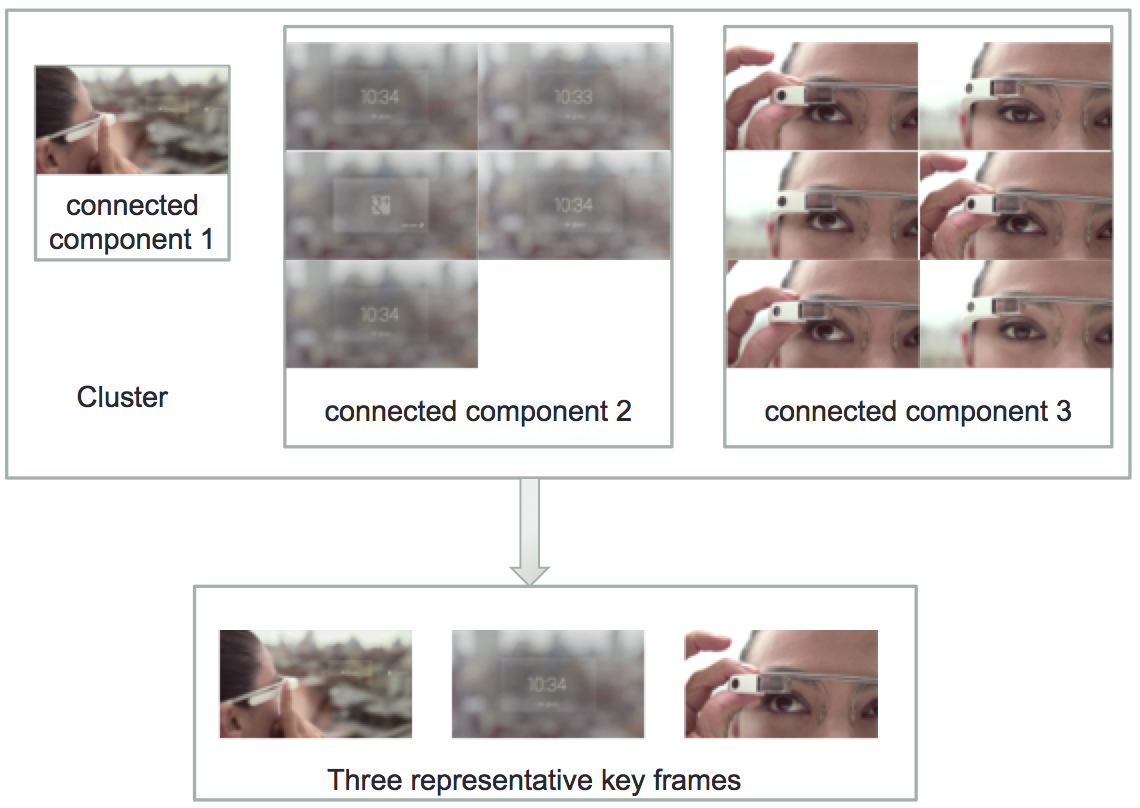
\includegraphics[scale = 0.6]{./keyFrames.png}
  \caption{Key frames identification example. In this cluster, there are three connected components. One frame is selected from each connected component. The resulting three frames are treated as representative frames.}
  \end{figure}

\noindent By combining all representative frames from all clusters, a video could be represented by those key frames. Therefore, the size of video is decreased to some degree and thus accelerates the process of recognition. 


